\documentclass[../the.tex]{subfiles}
\begin{document}
{\fontsize{13}{12} \selectfont

Trong phạm vi nghiên cứu này sẽ sử dụng mô hình Yolov7, Yolov8, SSD MobileNet. Mục \ref{sec:model} giới thiệu về các mô hình được sử dụng. Mục \ref{sec:dataset} mô tả về tập dữ liệu, và sơ đồ hệ thống ở Mục \ref{sec:sodo}

}
\section{Tập dữ liệu}
\label{sec:dataset}

{\fontsize{13}{12} \selectfont

	Trong phạm vi nghiên cứu, các tập dữ liệu sử dụng sẽ là TrashNet \cite{yang2016classification}, Taco \cite{proença2020taco} và bổ sung tập dữ liệu tự thu thập được ở ĐBSCL.
	Tham khảo việc phân loại rác của Yan \cite{yang2016classification} và quá trình thu thập dữ liệu thực tế nhận thấy các loại rác bằng thủy tinh ở môi trường bên ngoài rất thường là các mảnh kính trong suốt nhìn thấy nên hoặc có độ phản chiếu ánh sáng cao nên rất khó phát hiện, vì vậy các thủy tinh sẽ được gom vào các loại rác khác.
	Lớp giấy và thùng giấy sẽ được gom lại vì cùng chất liệu. Cuối cùng mô hình sẽ phân các loại ra làm các lớp:
	\begin{itemize}
		\item Kim loại gồm chủ yếu là các nắp bia, các vỏ bình làm bằng kim loại.
		\item Nhựa - nilon rất phổ biến, gồm các vật liệu làm từ nhựa như ly nhựa, các túi nilon.
		\item Giấy gồm các vật liệu từ giấy, các thùng giấy, vỏ gói thuốc lá, hộp giấy.
		\item Rác khác là các loại rác còn lại với từng loại xuất hiện ít hoặc khó phát hiện như thủy tinh, các vỏ gói đa sắc,
		      mút, vải,\dots
	\end{itemize}
}

\subsection{TrashNet}
\label{sec:trashnet}
{\fontsize{13}{12} \selectfont

	TrashNet là tập dữ liệu được giới thiệu trong bài nghiên cứu của \cite{yang2016classification} bao gồm các lớp và số lượng như bảng \ref{tab:dataset}. Tất cả hình ảnh được chụp bằng điện thoại Iphone7 sử dụng ánh sáng mặt trời hoặc ánh sáng phòng, các đối tượng được chụp trong nền trắng hoặc bao quát toàn bộ khung hình, một số hình ảnh ở tập Trashnet ở hình
	\ref{fig:dataset_0}.
	Do mục đích ban đầu của tập dữ liệu dùng để phân lớp nên nghiên cứu phải thực hiện gán hộp giới hạn cho bộ dữ liệu để phù hợp với nhu cầu phát hiện đối tượng. Tập dữ liệu TrashNet bao gồm các đối tượng có kích thước lớn và rõ ràng, mục đích sử dụng tăng độ nhận dạng cho mô hình. Bảng \ref{tab:dataset1} thể hiện số lượng đối tượng sau khi đã gán hộp giới hạn cho tập dữ liệu, hình
	\ref{fig:dataset_1} mô tả tập dữ liệu TrashNet khi được gán hộp giới hạn.

}

\begin{table}[!ht]
	\centering
	\caption{Số lượng ảnh theo lớp của tập dữ liệu TrashNet}
	\begin{tabular}{|l|l|r|}
		\hline
		\multicolumn{1}{|l|}{
			\textbf{\#}}
		 & \multicolumn{1}{c|}{\textbf{Lớp}}
		 & \multicolumn{1}{c|}{\textbf{Số lượng ảnh}} \\
		\hline

		1
		 & Cardboard
		 & 403                                        \\
		\hline

		2
		 & Paper
		 & 594                                        \\
		\hline

		3
		 & Glass
		 & 501                                        \\
		\hline

		4
		 & Plastic
		 & 482                                        \\
		\hline

		5
		 & Metal
		 & 410                                        \\
		\hline

		6
		 & Trash
		 & 137                                        \\
		\hline


		\textbf{Tổng cộng}
		 &
		 & 2524                                       \\
		\hline
	\end{tabular}

	\label{tab:dataset}
\end{table}

\begin{figure}[H]
	\centering
	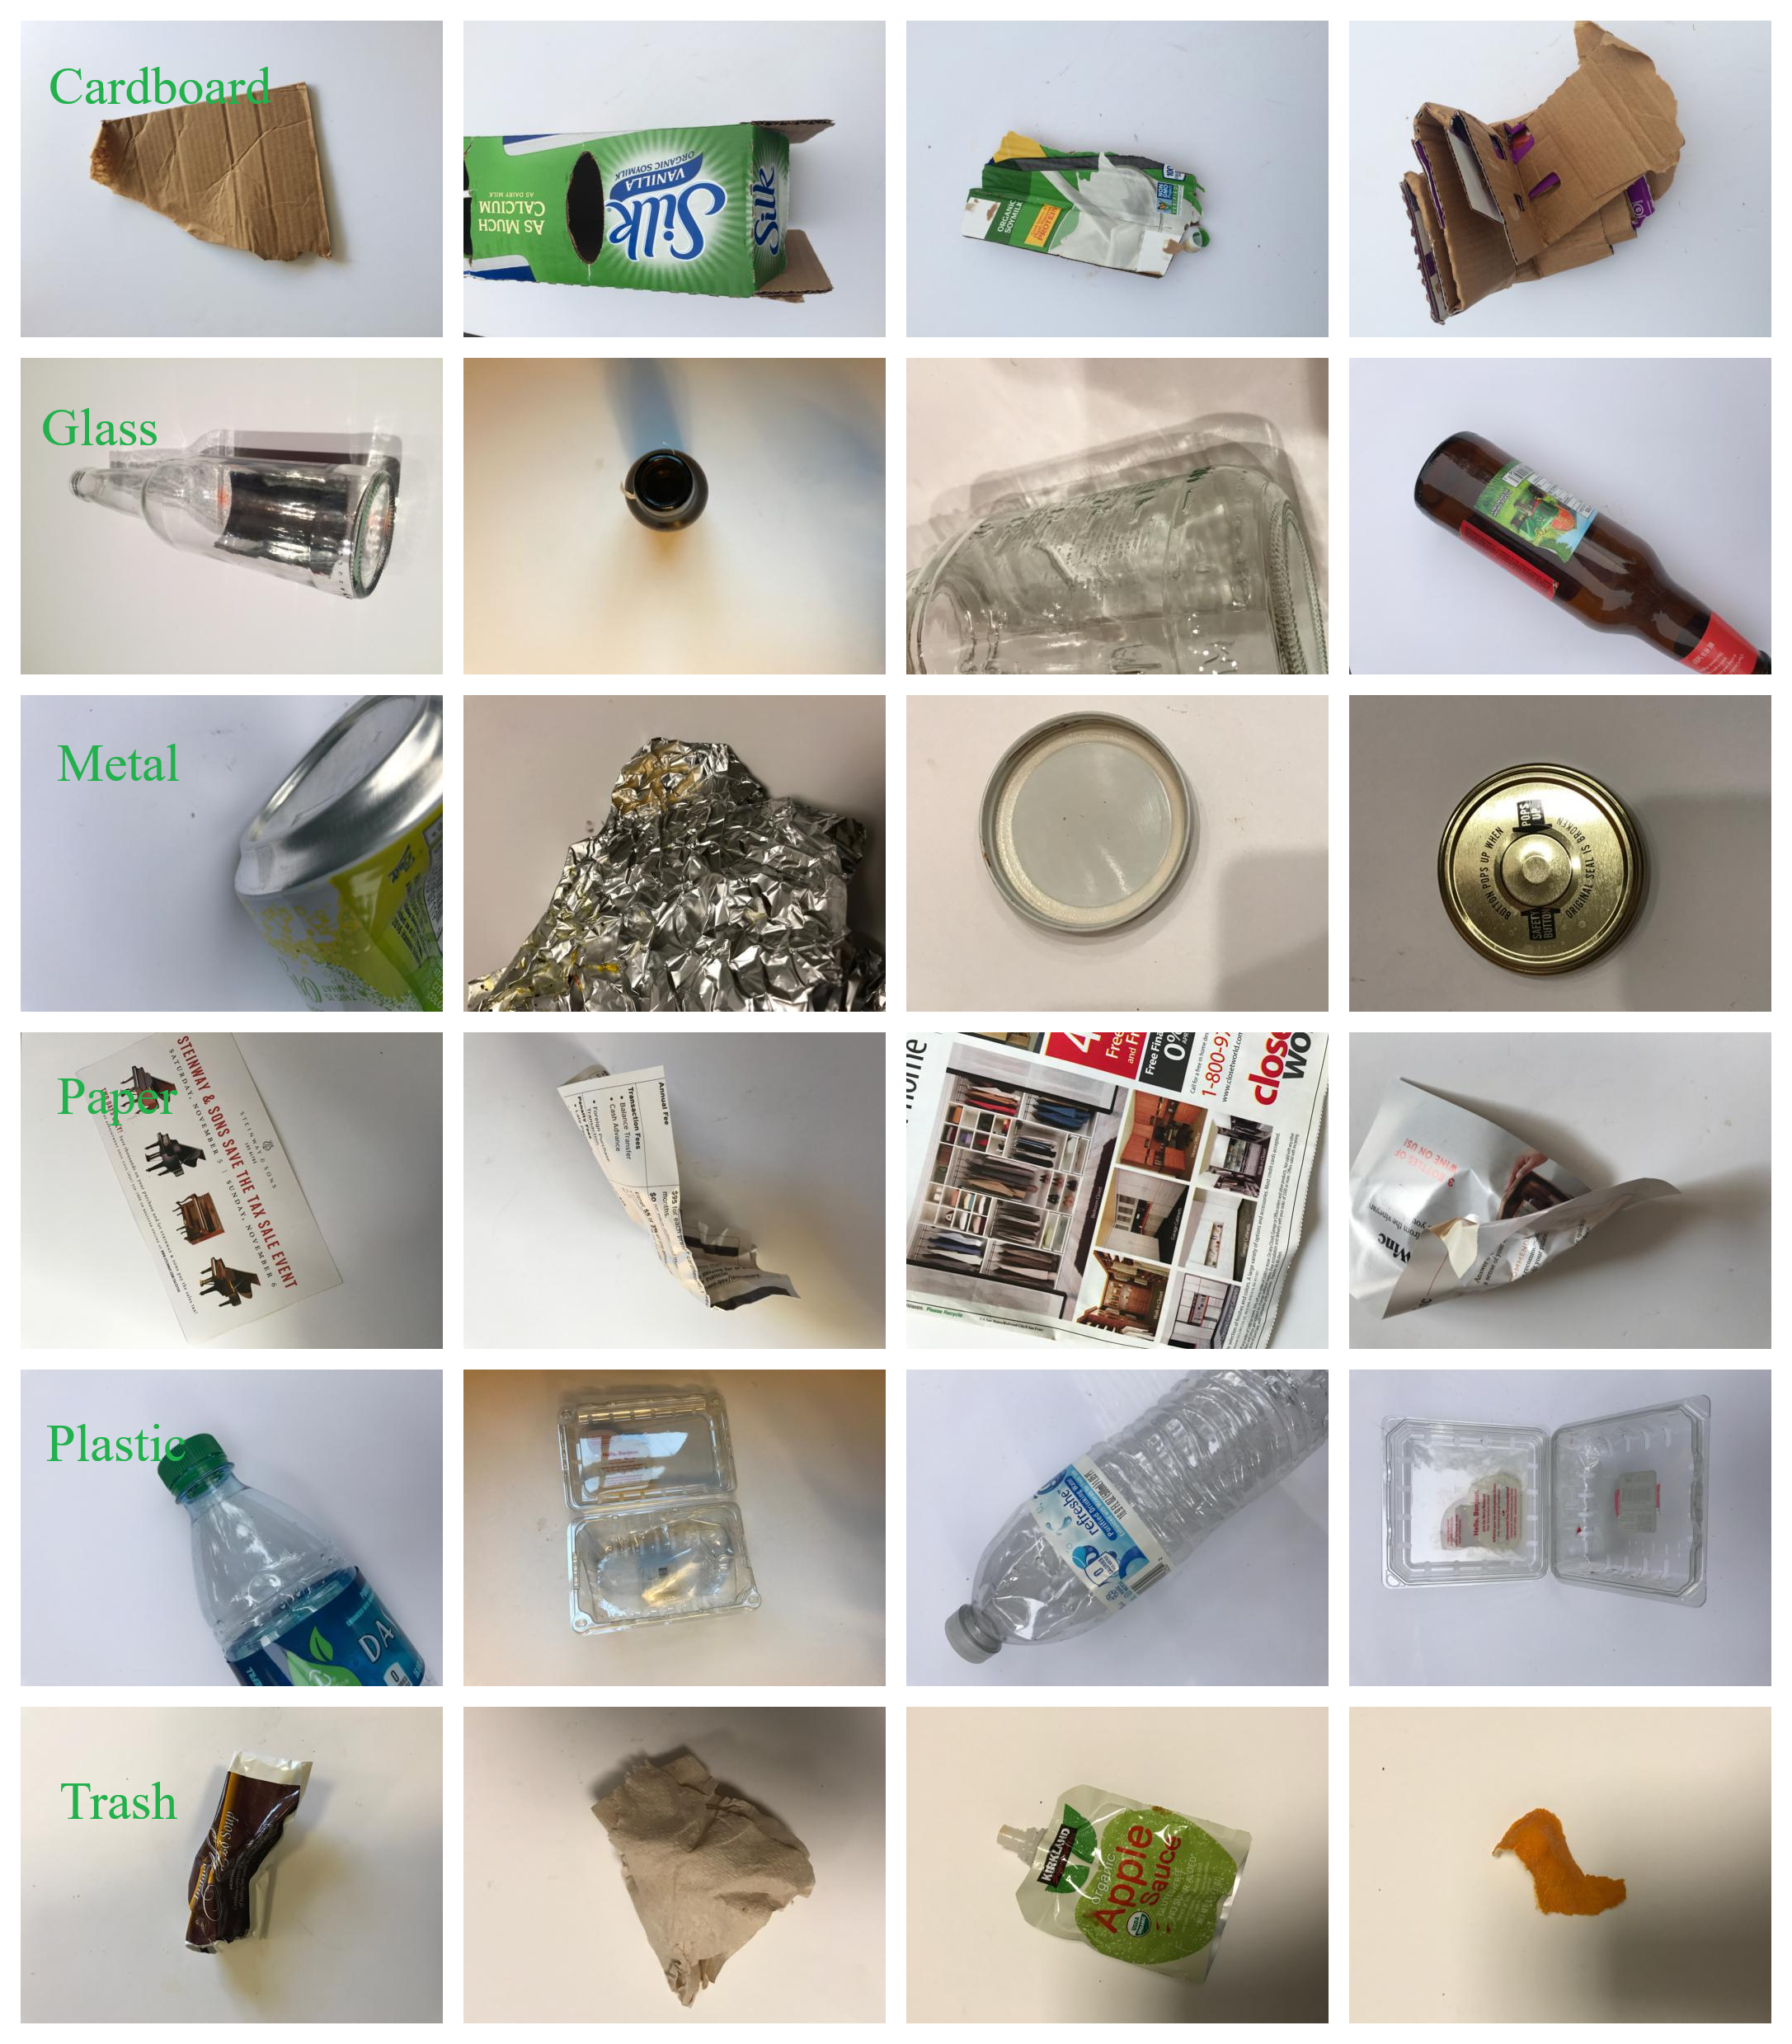
\includegraphics[width=1\textwidth]{trashnet_sample.png}
	\caption{Ví dụ về hình ảnh của tập dữ liệu TrashNet}
	\label{fig:dataset_0}
\end{figure}

\begin{table}[!ht]
	\centering
	\caption{Số lượng ảnh theo lớp của tập dữ liệu TrashNet khi được gán hộp giới hạn}
	\begin{tabular}{|l|l|r|}
		\hline
		\multicolumn{1}{|l|}{
			\textbf{\#}}
		 & \multicolumn{1}{c|}{\textbf{Lớp}}
		 & \multicolumn{1}{c|}{\textbf{Số lượng vật thể}} \\
		\hline

		1
		 & Cardboard
		 & 404                                            \\
		\hline

		2
		 & Paper
		 & 601                                            \\
		\hline

		3
		 & Glass
		 & 509                                            \\
		\hline

		4
		 & Plastic
		 & 479                                            \\
		\hline

		5
		 & Metal
		 & 410                                            \\
		\hline

		6
		 & Trash
		 & 149                                            \\
		\hline


		\textbf{Tổng cộng}
		 &
		 & 2552                                           \\
		\hline
	\end{tabular}

	\label{tab:dataset1}
\end{table}

\begin{figure}[H]
	\centering
	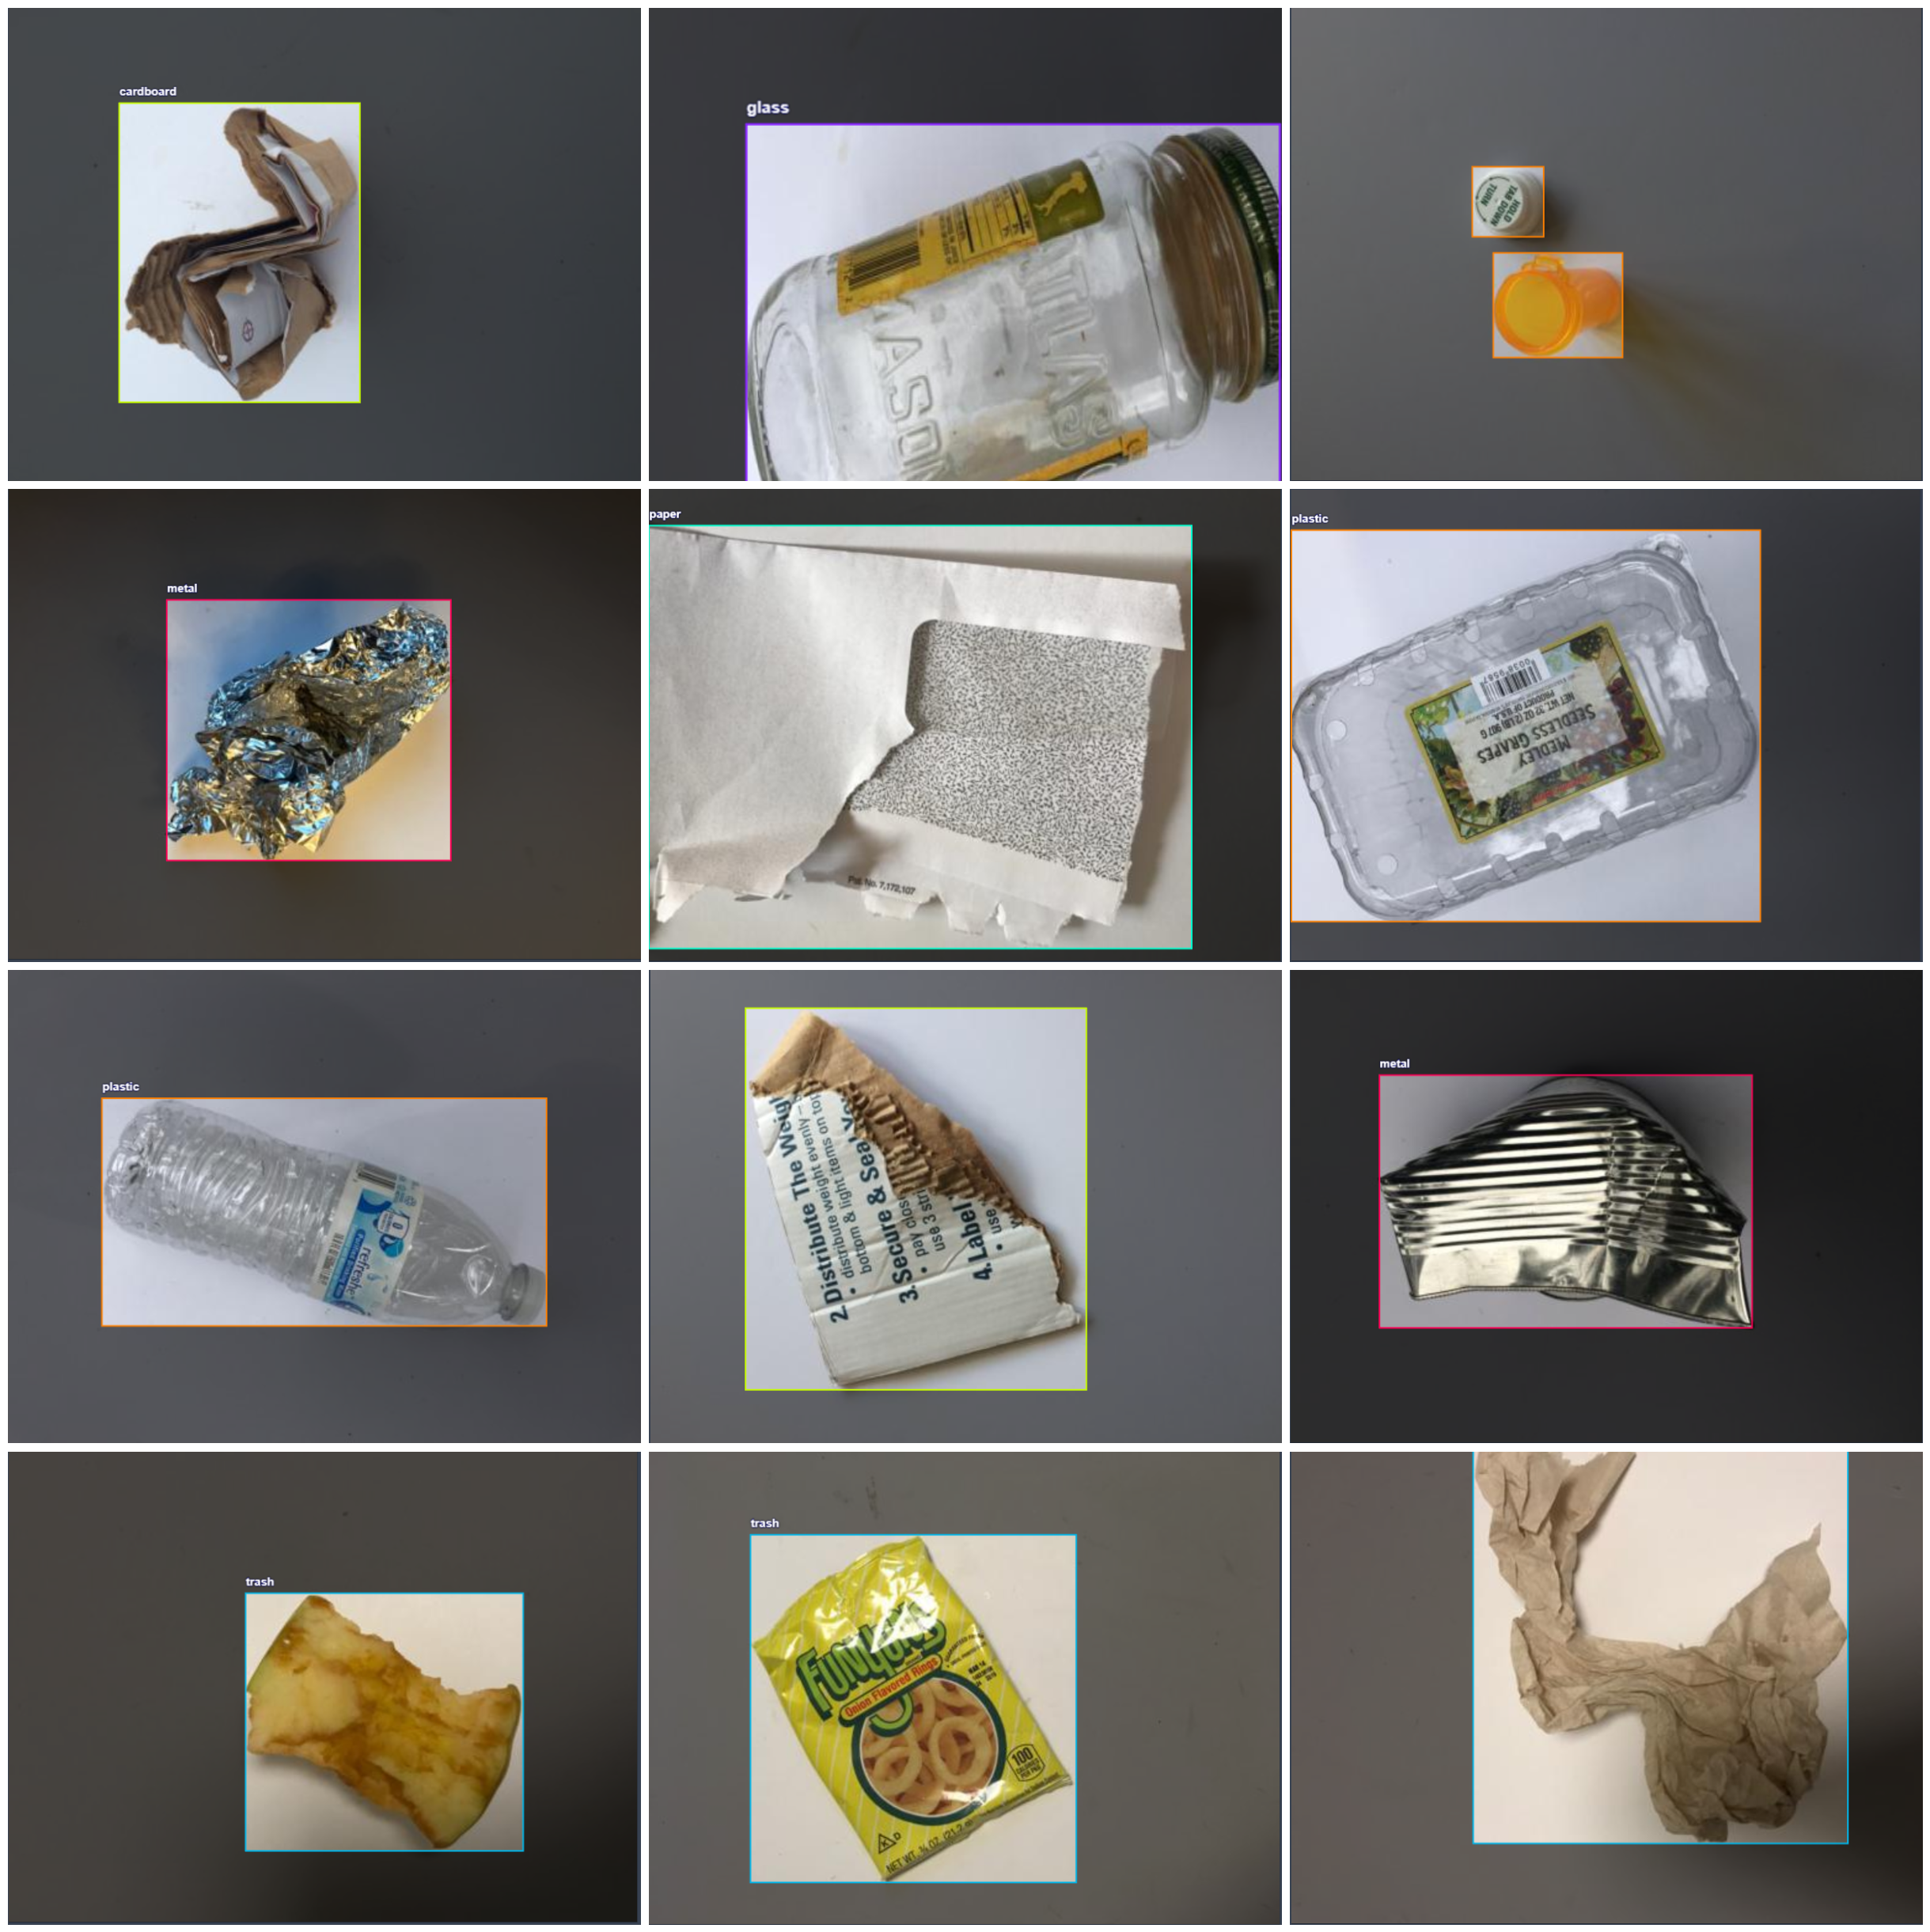
\includegraphics[width=1\textwidth]{trashnet_sample2.png}
	\caption{Ví dụ về hình ảnh của tập dữ liệu TrashNet được gán hộp giới hạn}
	\label{fig:dataset_1}
\end{figure}

\subsection{Taco}
\label{sec:Taco}
{\fontsize{13}{12} \selectfont

	Taco là một tập dữ liệu hình ảnh về chất thải trong tự nhiên. Tập dữ liệu chứa các hình ảnh về rác được chụp trong nhiều môi trường khác nhau, từ những bãi biển đến đường phố London. Những hình ảnh này được gắn nhãn và phân đoạn thủ công để đào tạo và đánh giá các thuật toán phát hiện đối tượng.
	Bộ dữ liệu được cung cấp
	theo chuẩn json của COCO. Hiện tại bộ dữ liệu có 1.500 ảnh với 4.784 vật thể
	và 3918 ảnh mới cần được gán nhãn.

}

\begin{figure}[H]
	\centering
	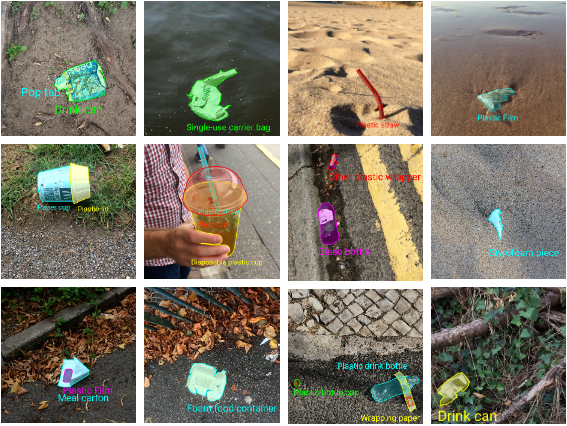
\includegraphics[width=1\textwidth]{Taco.png}
	\caption{Ví dụ về hình ảnh của bộ dữ liệu Taco \cite{proença2020taco}}
	\label{fig:dataset_taco}
\end{figure}
{\fontsize{13}{12} \selectfont

Bộ dữ liệu gồm 28 danh mục lớn  (xem Hình \ref{fig:dataset_taco_1_a}) và 60 danh mục nhỏ (xem Hình \ref{fig:dataset_taco_1_b}) với
6 loại nền là rác, thảm cỏ, nước, trong nhà, vỉa hè, cát đá (xem Hình \ref{fig:dataset_taco_1_c}). Do
điều kiện đường phố ở một số tỉnh ĐBSCL nên nghiên cứu loại bỏ ngữ cảnh trong nhà, cát đá và nước phục vụ cho mục đích huấn luyện mô hình. Các danh
mục nhỏ được gom nhóm phù hợp thành bốn loại rác đề ra của nghiên cứu như Bảng \ref{tab:taco_map}. Bộ dữ liệu Taco thể hiện sự đa dạng trong từng loại rác,
tuy nhiên đó cũng là sự hạn chế khi có những lớp có quá ít dữ liệu như Carded blister pack (1 đối tượng), Battery (2 đối tượng), và các lớp có quá nhiều đối tượng như Cigarette (667 đối tượng) và Unlabeled litter (516 đối tượng).

}

\begin{figure}[H]
	\centering
	\subfloat[\centering {\fontsize{11}{10} \selectfont Danh mục lớn }]{{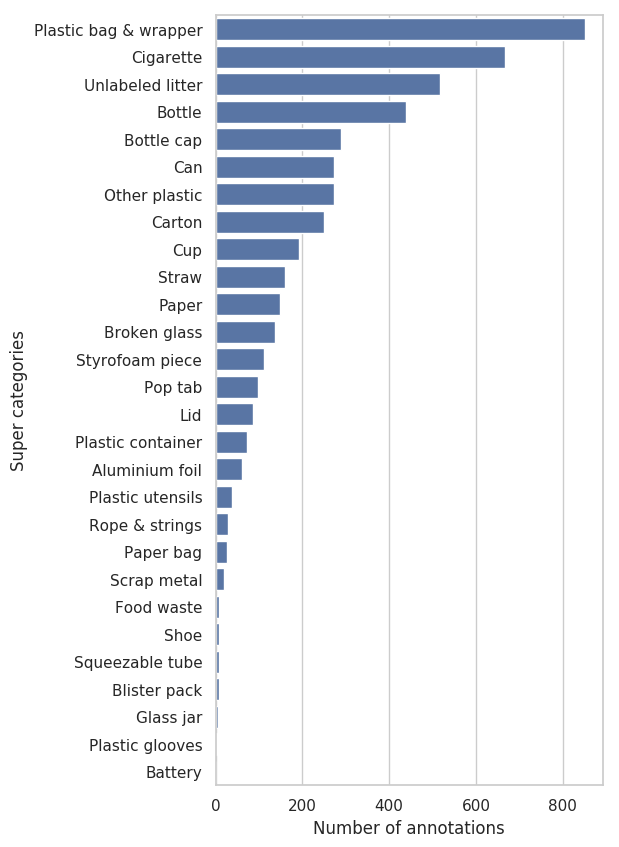
\includegraphics[width=7cm]{taco_super.png} \label{fig:dataset_taco_1_a}}}%
	\qquad
	\subfloat[\centering {\fontsize{11}{10} \selectfont Danh mục nhỏ}]{{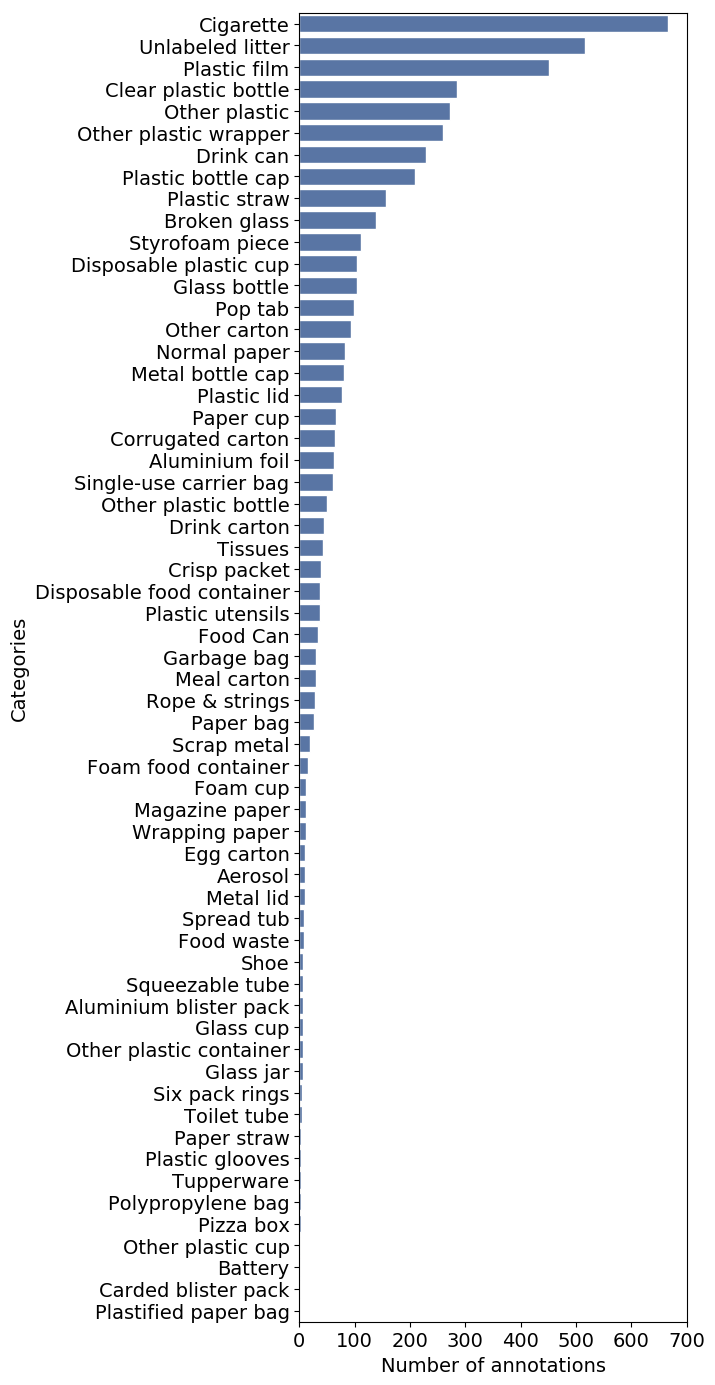
\includegraphics[width=7cm]{taco_cat.png} \label{fig:dataset_taco_1_b}}}%
	\qquad
	\subfloat[\centering {\fontsize{11}{10} \selectfont Tỉ lệ nền}]{{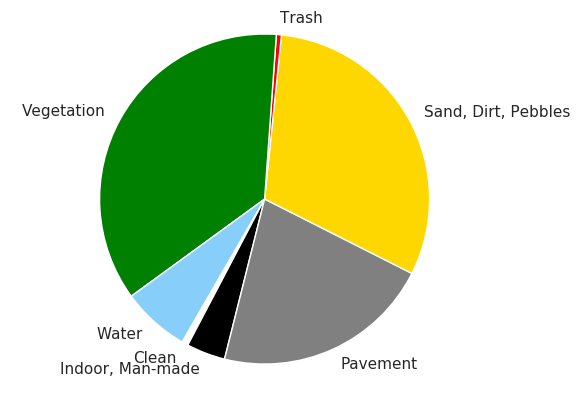
\includegraphics[width=10cm]{taco_bg.png} \label{fig:dataset_taco_1_c}}}%
	\caption{Các thống kê theo danh mục lớn, danh mục nhỏ, tỉ lệ nền của bộ dữ liệu Taco}%
	\label{fig:dataset_taco_1}
\end{figure}

\begin{table}[!ht]
	\centering
	\caption{Bảng chuyển các lớp của Taco sang lớp của mô hình}
	\begin{tabular}{|l|l|l|l|}
		\hline
		\multicolumn{1}{|c|}{\textbf{Taco}}
		                       & \multicolumn{1}{c|}{\textbf{Mô hình}}
		                       & \multicolumn{1}{c|}{\textbf{Taco}}
		                       & \multicolumn{1}{c|}{\textbf{Mô hình}}                                           \\
		\hline
		Aluminium foil         & kim\_loai                             & Magazine paper            & giay        \\ \hline
		Battery                & kim\_loai                             & Tissues                   & giay        \\ \hline
		Aluminium blister pack & khac                                  & Wrapping paper            & giay        \\ \hline
		Carded blister pack    & khac                                  & Normal paper              & giay        \\ \hline
		Other plastic bottle   & nhua\_nilon                           & Paper bag                 & giay        \\ \hline
		Clear plastic bottle   & nhua\_nilon                           & Plastified paper bag      & giay        \\ \hline
		Glass bottle           & khac                                  & Plastic film              & nhua\_nilon \\ \hline
		Plastic bottle cap     & nhua\_nilon                           & Six pack rings            & khac        \\ \hline
		Metal bottle cap       & kim\_loai                             & Garbage bag               & nhua\_nilon \\ \hline
		Broken glass           & khac                                  & Other plastic wrapper     & nhua\_nilon \\ \hline
		Food Can               & kim\_loai                             & Single-use carrier bag    & nhua\_nilon \\ \hline
		Aerosol                & kim\_loai                             & Polypropylene bag         & nhua\_nilon \\ \hline
		Drink can              & kim\_loai                             & Crisp packet              & khac        \\ \hline
		Toilet tube            & giay                                  & Spread tub                & nhua\_nilon \\ \hline
		Other carton           & giay                                  & Tupperware                & nhua\_nilon \\ \hline
		Egg carton             & giay                                  & Disposable food container & nhua\_nilon \\ \hline
		Drink carton           & giay                                  & Foam food container       & giay        \\ \hline
		Corrugated carton      & giay                                  & Other plastic container   & nhua\_nilon \\ \hline
		Meal carton            & giay                                  & Plastic glooves           & nhua\_nilon \\ \hline
		Pizza box              & giay                                  & Plastic utensils          & nhua\_nilon \\ \hline
		Paper cup              & giay                                  & Pop tab                   & kim\_loai   \\ \hline
		Disposable plastic cup & nhua\_nilon                           & Rope \& strings           & khac        \\ \hline
		Foam cup               & giay                                  & Scrap metal               & kim\_loai   \\ \hline
		Glass cup              & khac                                  & Shoe                      & khac        \\ \hline
		Other plastic cup      & nhua\_nilon                           & Squeezable tube           & khac        \\ \hline
		Food waste             & khac                                  & Plastic straw             & nhua\_nilon \\ \hline
		Glass jar              & khac                                  & Paper straw               & nhua\_nilon \\ \hline
		Plastic lid            & nhua\_nilon                           & Styrofoam piece           & khac        \\ \hline
		Metal lid              & kim\_loai                             & Unlabeled litter          & khac        \\ \hline
		Other plastic          & nhua\_nilon                           & Cigarette                 & khac        \\ \hline
	\end{tabular}
	\label{tab:taco_map}
\end{table}

\subsection{Dữ liệu tự thu thập}
\label{sec:own}
{\fontsize{13}{12} \selectfont

	Hình \ref{fig:dataset_own} là bộ dữ liệu được thực hiện lấy mẫu ở các tỉnh thành ở ĐBSCL như Cần Thơ, Vĩnh Long và chủ yếu ở Trà Vinh nhầm phản ánh thực tế tình trạng rác ở địa phương.
	Dữ liệu thu thập gồm 663 hình ảnh với 1766 đối tượng được chia cho bốn lớp kim loại, nhựa - nilon, giấy, rác khác với trung bình 2.6 đối tượng mỗi hình ảnh (bảng \ref{tab:datasetown}).
	Phần lớn là các hộp thức ăn giấy, các bọc nilon, ly nhựa, túi rác, khẩu trang giấy và các phần rác cũ không có hình dạng cố định.
	Việc thu thập thêm dữ liệu nhầm giúp mô hình học tập và cải thiện khả năng phát hiện đúng thực tế. Trong quá trình thực hiện thu thập dữ liệu gặp những vấn đề như sau:

	\begin{itemize}
		\item Các rác chồng chéo khó xác định hộp giới hạn.
		\item Tình trạng rác cũ, rác nhỏ bị ẩn vào nền, rất khó xác định nhãn.
		\item Xuất hiện các đối tượng rác có thể gồm nhiều nhãn. Ví dụ như túi nilon chứa bọc giấy, lon kim loại, các gói sắc nét hộp thức ăn nhựa trong suốt chứa rác hữu cơ.
		\item Phần rác kim loại xuất hiện ít, vì hầu hết được người dân xử lí chủ động trước. Tuy nhiên phần rác kim loại vẫn có đặc tính dễ phát hiện và bổ sung dữ liệu từ Taco \cite{proença2020taco} và TrashNet.
		\item Các loại còn lại được gom vào rác khác sẽ giảm khả năng phân lớp vì độ đa dạng cao.
	\end{itemize}

}

\begin{table}[!ht]
	\centering
	\caption{Số lượng ảnh, đối tượng và tỉ lệ theo lớp của tập dữ liệu tự thu thập}
	\begin{tabular}{|l|r|r|r|}
		\hline
		\multicolumn{1}{|c|}{\textbf{Lớp}}
		                  & \multicolumn{1}{c|}{\textbf{Số hình}}
		                  & \multicolumn{1}{c|}{\textbf{Số đối tượng}}
		                  & \multicolumn{1}{c|}{\textbf{Tỉ lệ}}
		\\
		\hline

		Nhựa - Nilon      & 392                                      & 761 & 43.1\% \\
		\hline

		Giấy              & 339                                      & 552 & 31.3\% \\
		\hline

		Rác khác          & 209                                      & 350 & 19.8\% \\
		\hline

		Kim loại          & 60                                       & 103 & 5.8\%  \\
		\hline
		Ảnh không vật thể & 200                                      & 0   & 0      \\
		\hline
	\end{tabular}

	\label{tab:datasetown}
\end{table}

{\fontsize{13}{12} \selectfont

Bảng \ref{tab:datasetown} thể hiện rác thải nhựa-nilon chiếm phần lớn các loại rác ở đường phố hiện nay và rác kim loại rất ít chỉ khoảng 5,8\% dữ liệu thu thập được.
Việc mất cân bằng dữ liệu ở tập dữ liệu tự thu thập sẽ được bổ sung bằng các tập dữ liệu của Taco và TrashNet, từ đó tạo ra bộ dữ liệu để huấn luyện và kiểm thử.
Ngoài ra nghiên cứu còn thu thập thêm 200 hình ảnh nền để tăng cường dữ liệu, đặt ra vấn đề các ảnh nền không chứa đối tượng nào (background) có tăng khả năng nhận diện của mô hình bằng cách giảm việc nhận dạng sai các đối tượng không phải là rác hay không.

}


\begin{figure}[H]
	\centering
	\includegraphics[width=1\textwidth]{data_own.png}
	\caption{Ví dụ về bộ dữ liệu thu thập}
	\label{fig:dataset_own}
\end{figure}

\subsection{Dữ liệu sử dụng cho mô hình}
{\fontsize{13}{12} \selectfont

	Trong phạm vi nghiên cứu sẽ sử dụng kết hợp giữa các bộ dữ liệu được nêu ở Mục \ref{sec:trashnet}, \ref{sec:Taco}, \ref{sec:own} để tạo ra các bộ dữ liệu phù hợp với các mục đích huấn luyện.
	Tập dữ liệu Taco được tiền xử lí để loại bỏ đi những vật thể có kích thước quá nhỏ (dưới 0.005\%) so với hình, việc này nhằm loại bỏ những dữ liệu nhiễu và không thể phân loại rác.
	Nghiên cứu thực nghiệm trên các mô hình với nhiệm vụ phát hiện rác, sau đó vừa phát hiện vừa phân loại, tiếp theo là bổ sung dữ liệu nền để cải thiện mô hình.
	Bảng \ref{tab:datasetmain} trình bày sự kết hợp của cả ba bộ dữ liệu.

}

\begin{table}[!ht]
	\centering
	\caption{Số lượng hình ảnh, đối tượng của tập dữ liệu sử dụng cho nghiên cứu được tổng hợp từ dữ liệu TrashNet, Taco và tự thu thập}
	\begin{tabular}{|l|l|r|r|r|}
		\cline{1-5}
		\textbf{Lớp}                           &            &\textbf{TrashNet} & \textbf{Taco} & \textbf{Thu thập} \\ \cline{1-5}
		\multirow{2}{*}{\textbf{Nhựa - nilon}} & Hình ảnh   & 495               & 604           & 392               \\ \cline{2-5}
		                                       & Đối tượng  & 496               & 1252          & 761               \\ \cline{1-5}
		\multirow{2}{*}{\textbf{Giấy}}         & Hình ảnh   & 591               & 349           & 339               \\ \cline{2-5}
		                                       & Đối tượng  & 591               & 488           & 552               \\ \cline{1-5}
		\multirow{2}{*}{\textbf{Kim loại}}     & Hình ảnh   & 409               & 221           & 60                \\ \cline{2-5}
		                                       & Đối tượng  & 410               & 346           & 103               \\ \cline{1-5}
		\multirow{2}{*}{\textbf{Khác}}     & Hình   ảnh & 587               & 365           & 209               \\ \cline{2-5}
		                                       & Đối tượng  & 612               & 547           & 350               \\ \cline{1-5}
	\end{tabular}
	\label{tab:datasetmain}
\end{table}

{\fontsize{13}{12} \selectfont

Nghiên cứu sẽ sử dụng các bộ dữ liệu như sau:

\begin{itemize}
	\item Bộ dữ liệu 1 kết hợp của dữ liệu Taco, tự thu thập và bổ sung dữ liệu TrashNet để giải quyết vấn đề mất cân bằng dữ liệu. Tập dữ liệu dùng để thử nghiệm gồm hình ảnh rác trong tự nhiên được lấy từ Taco và tự thu thập, thể hiện ở Bảng \ref{tab:datasettest}
	      Trong đó, lớp "Unlabeled litter" của bộ dữ liệu Taco sẽ được gán lại nhãn thủ công để phù hợp với dữ liệu của nghiên cứu. Bảng \ref{tab:datasetmain} mô tả chi tiết các hình ảnh và đối tượng được sử dụng trong nghiên cứu được lấy từ việc kết hợp ba bộ dữ liệu.\label{item:dataset}
	\item Bộ dữ liệu 2 nhưng bổ sung 200 hình nền không có đối tượng.
\end{itemize}

}

\begin{table}[!ht]
	\centering
	\caption{Số lượng đối tượng theo từng lớp của tập huấn luyện, xác thực, thử nghiệm dùng trong nghiên cứu}
	\begin{tabular}{|l|r|r|r|}
		\cline{1-4}
		\textbf{Lớp}          & \textbf{Huấn luyện} & \textbf{Xác thực} & \textbf{Thử nghiệm}\\ \cline{1-4}
		\textbf{Nhựa - nilon} & 1656 & 618 & 235                \\ \cline{1-4}
		\textbf{Giấy}         & 1179 & 289 & 163                \\ \cline{1-4}
		\textbf{Kim loại}     & 660 & 150 & 49               \\ \cline{1-4}
		\textbf{Khác}         & 999 & 401 & 109               \\ \cline{1-4}
	\end{tabular}

	\label{tab:datasettest}
\end{table}

{\fontsize{13}{12} \selectfont

Việc gán nhãn cho dữ liệu ảnh hưởng đến hiểu quả mô hình vì rất dễ nhầm lẫn về định nghĩa rác theo thành phần. Ví dụ như các lớp được chuyển đổi từ bộ dữ liệu Taco (bảng \ref{tab:taco_map}).
Ngoài ra bộ dữ liệu Taco là do cộng đồng đóng góp, vì vậy việc xuất hiện nhiều lớp "Unlabeled litter" sẽ gây nhiễu cho dữ liệu, cần phải gán nhãn lại.
Tập dữ liệu để đánh giá mô hình chỉ gồm dữ liệu của \ref{sec:Taco} và \ref{sec:own} để đánh giá khả năng phát hiện thực tế của mô hình ở điều kiện tự nhiên.

}
% Please add the following required packages to your document preamble:
% \usepackage{multirow}
% Please add the following required packages to your document preamble:
% \usepackage{multirow}


\section{Các mô hình sử dụng}
\label{sec:model}
\subsection{Mô hình Yolov7}
{\fontsize{13}{12} \selectfont

	Mô hình Yolov7 được trình bày cơ bản ở Mục \ref{sec:yolov7}, trong phần này sẽ giới thiệu kiến trúc được sử dụng trong nghiên cứu. Mô hình cài đặt sẽ nhận ảnh kích thước đầu vào là 640x640, sử dụng phiên bản Yolov7-p5. Kiến trúc Yolov7 (xem Hình \ref{fig:yolov7_kientruc}) sử dụng:
	\begin{itemize}
		\item Backbone: ELAN giải quyết vấn đề hội tụ khi thực hiện model scaling. ELAN được tạo từ các khối ELANBlock chịu ảnh hưởng từ CSPNet \cite{wang2019cspnet} và VoVNet \cite{lee2019energy}, các ELANBlock sẽ được kết nối với nhau thông qua Transition Block để giảm kích cỡ của bản đồ đặc trưng xuống hai lần.
		\item Neck: CSPSPP + PANet. CSPSPP (Cross Stage Partial Spatial Pyramid Pooling) được sử dụng trong Yolov7 giúp xử lý ảnh có kích thước khác nhau từ nhiều nguồn, trích xuất được cái đặc trưng từ nhiều tỷ lệ và bảo toàn được vị trí các vật thể. CSPSPP làm tăng độ phức tạp của mô hình so với các mạng gộp đơn giản.
		\item Head: YOLOR. Cấu trúc của head trong YOLOv7
		      gồm 3 lớp mạng nơ-ron hoàn toàn kết nối
		      (fully-connected layers). Lớp thứ nhất
		      là dự đoán các ô lưới (grid cells) chứa đối
		      tượng. Lớp thứ hai là dự đoán các hộp giới hạn cho các đối tượng. Lớp thứ ba dự đoán lớp của đối tượng \cite{cachuayol7}.
	\end{itemize}

}

\begin{figure}[H]
	\centering
	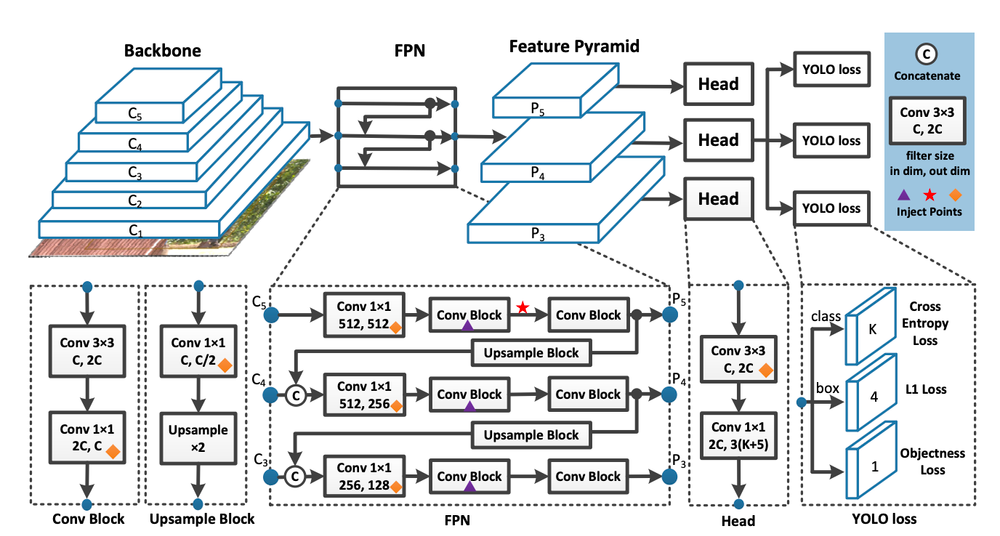
\includegraphics[width=0.8\textwidth]{yolov7_kientruc.jpg}
	\caption{Kiến trúc mô hình Yolov7}
	\label{fig:yolov7_kientruc}
\end{figure}

\subsection{Mô hình Yolov8}
{\fontsize{13}{12} \selectfont

	Như Mục \ref{sec:yolov8} đã trình bày những thay đổi mới của yolov8 mang lại. Yolov8 vẫn nhận hình ảnh đầu vào là 640x640, sử dụng phiên bản Yolov8n. Kiến trúc của Yolov8 như sau:
	\begin{itemize}
		\item Backbone: là nền tảng của Yolov8, có nhiệm vụ trích xuất cái đặc trưng từ ảnh đầu vào. Yolov8 sử dụng CSPDarknet53, một biến thể của mạng Darknet làm backbone.
		      Kiến trúc CSPDarknet53 sử dụng Cross-Stage Partial (CSP) để cải thiện luồng thông tin và cải thiện độ chính xác.
		\item Neck: PANet. Phần neck có nhiệm vụ kết hợp các bản đồ đặc trưng để nắm bắt thông tin ở nhiều tỉ lệ khác nhau. Yolov8 sử dụng module C2f thay vì C3 gồm hai lớp tích chập kết hợp với CSP giúp xử lí nhanh hơn, cải thiện khả năng phát hiện các vật thể nhỏ.
		\item Head: gồm nhiều head giúp phát hiện, mỗi head chịu trách nhiệm dự đoán hộp giới hạn, xác suất của lớp và vị trí các đối tượng ở tỉ lệ  khác nhau.
		      gồm 3 lớp mạng nơ-ron hoàn toàn kết nối
		      (fully-connected layers). Lớp thứ nhất
		      là dự đoán các ô lưới (grid cells) chứa đối
		      tượng. Lớp thứ hai là dự đoán các hộp giới hạn cho các đối tượng. Lớp thứ ba dự đoán lớp của đối tượng.
	\end{itemize}

}

\begin{figure}[H]
	\centering
	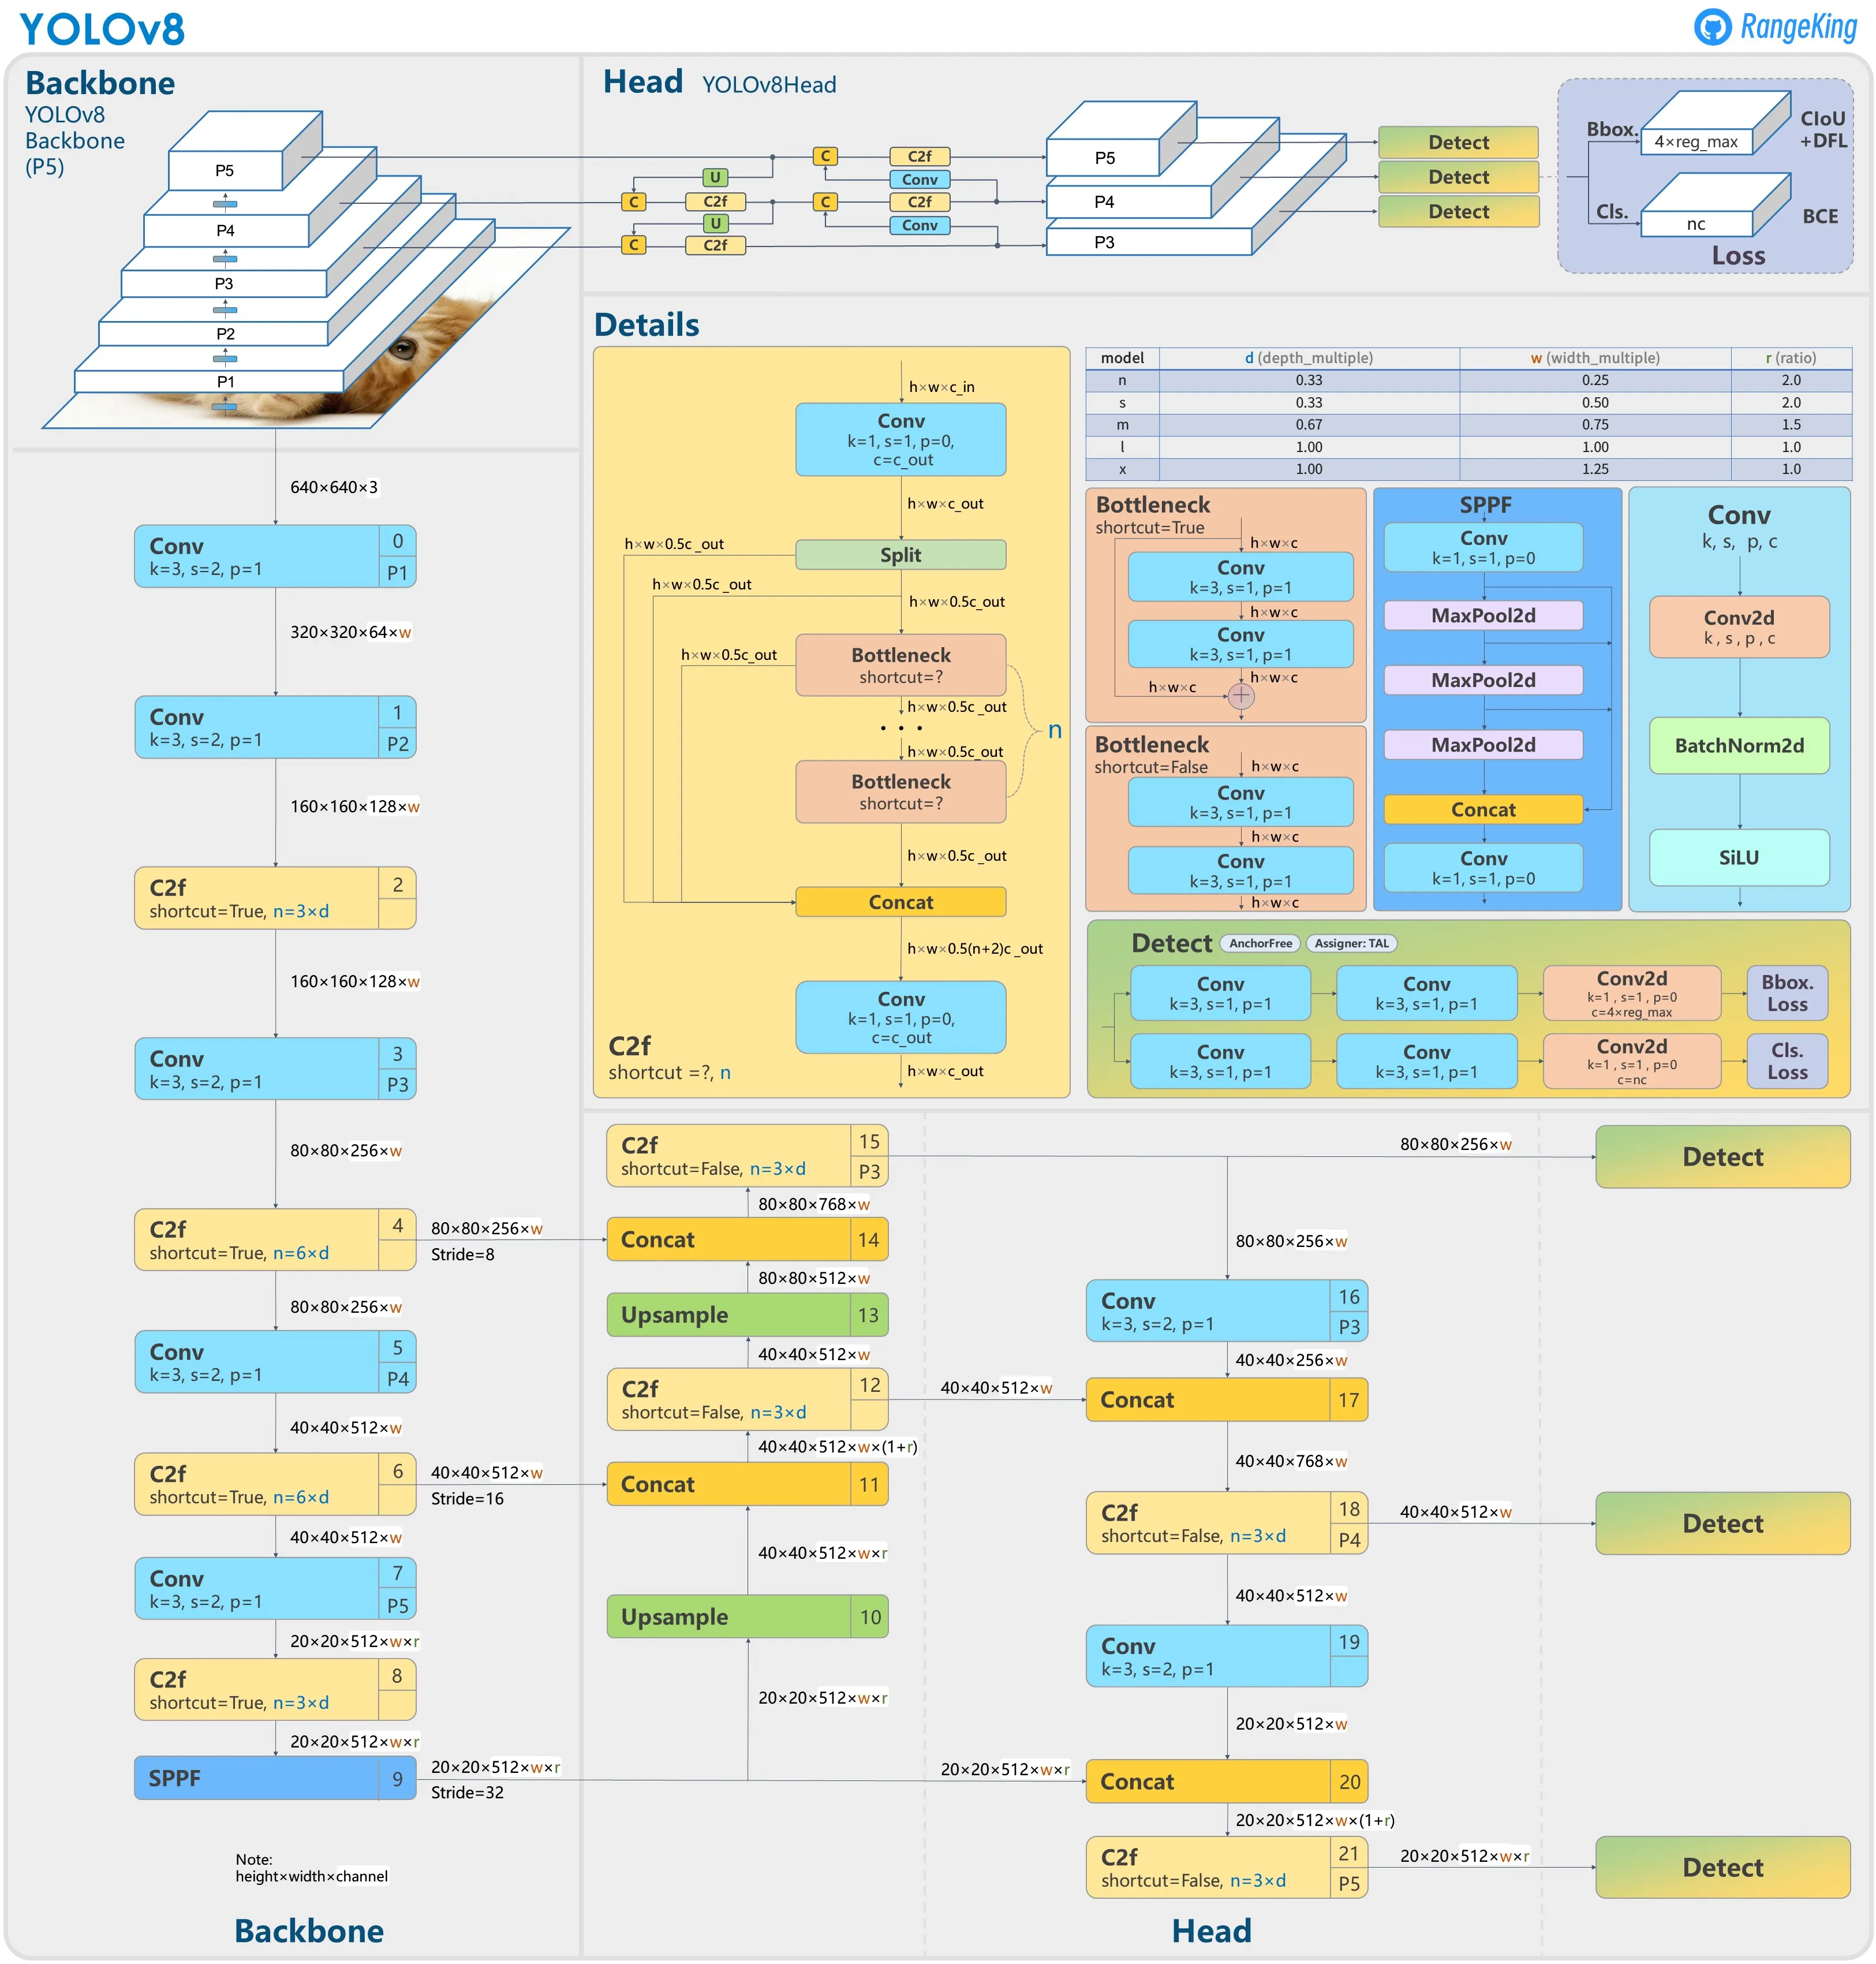
\includegraphics[width=0.8\textwidth]{yolov8_kientruc.jpg}
	\caption{Kiến trúc mô hình Yolov8 trên github được đóng góp bởi RangeKing}
	\label{fig:yolo8_kientruc}
\end{figure}

{\fontsize{13}{12} \selectfont

Với những cải tiến của Yolov8 mang lại như giảm kích thước mạng tích chập từ $6x6$ xuống $3x3$ để trừu tượng hoá hình ảnh hiệu quả, thay thế module C3 bằng module C2f tăng tốc độ xử lí, triển khai dự đoán không cần hộp neo để loại bỏ sự cần thiết của hộp neo,
tận dụng các kỹ thuật tăng cường dữ liệu khác nhau để cải thiện khả năng tổng quát hóa và giảm tình trạng trang bị quá mức, sử dụng hàm mất mát được sửa đổi (tác giả không giới thiệu) tập trung vào hộp giới hạn và độ tin cậy khi phân lớp.
Nghiên cứu sử dụng Yolov7 và Yolov8 để so sánh độ hiệu quả của hai mô hình mới nhất của họ Yolo, hai mô hình có sự khác biệt về kiến trúc mạng, hàm mất mát và việc sử dụng hay không sử dụng hộp neo.

}

\subsection{Mô hình SSD MobileNetv2}
{\fontsize{13}{12} \selectfont

	Phần \ref{sec:ssd} đã giới thiệu về kiến trúc tổng quan của mô hình SSD. Trong nghiên cứu sử dụng MobiNetv2 \cite{sandler2019mobilenetv2} làm mạng cơ sở thay vì VGG-16 như Hình \ref{fig:ssd2} giúp tối ưu hóa cho các thiết bị di động. SSD MobileNetv2 sử dụng MobileNetv2 để trích xuất các tính năng từ ảnh, sau đó được xử lí thông qua các lớp dự đoán của SSD để giảm kích thước hình ảnh, giúp nhận ra các đối tượng ở tỉ lệ khác nhau (xem Hình \ref{fig:mobinet}).
	Mô hình MobiNet ra đời dựa vào nhu cầu tăng cao về các mô hình có trọng số nhẹ, giải quyết bài toán sử dụng trên các thiết bị hạn chế về tài nguyên tính toán như mobile, IoT. MobiNet có độ chính xác không chênh lệch so với mạng cơ sở VGG, nên việc thay thế trong kiến trúc của SSD giúp cho mô hình vừa nhỏ gọn vừa đạt độ chính xác cao.
	Điểm cải tiến của MobiNet là việc sử dụng tích chập tách biệt chiều sâu thay vì tích chập thông thường. Quá trình được phân chia làm hai bước tuần tự là tích chập chiều sâu và tích chập điểm.
	MobiNetv2 được nhóm tác giả giới thiệu với module mới được gọi là Inverted Residual Block đi ngược lại với các Residual Block thông thường vì nó tăng độ sâu trước khi học các đặc trưng, MobileNetv2 còn sử dụng hàm kích hoạt tuyến tính thay vì hàm kích hoạt phi tuyến.

}

\begin{figure}[H]
	\centering
	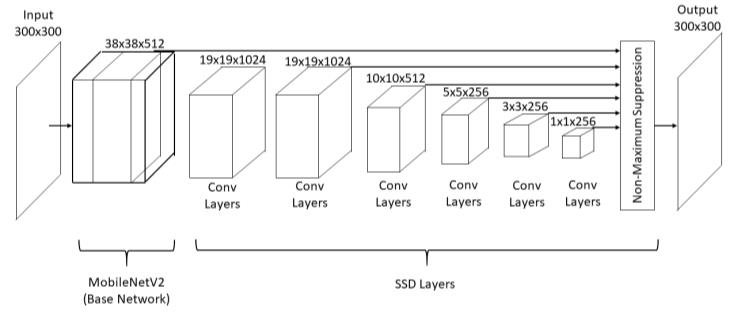
\includegraphics[width=0.8\textwidth]{mobinet.png}
	\caption{Kiến trúc mô hình SSD MobileNetv2}
	\label{fig:mobinet}
\end{figure}

\section{Sơ đồ hệ thống}
\label{sec:sodo}
{\fontsize{13}{12} \selectfont

	Các bước xây dựng hệ thống được chia làm hai giai đoạn được mô tả ở Hình \ref{fig:sodo}:

	\begin{itemize}
		\item Tiến hành thu thập dữ liệu và kết hợp dữ liệu như đã đề ra ở Mục \ref{sec:dataset}, sau đó dữ liệu được huấn luyện và đánh giá với các mô hình ở Mục \ref{sec:model} để tìm ra mô hình tối ưu cho hệ thống.
		      Qua trình huấn luyện mô hình thực hiện dựa trên các thư viện, dự án như Ultralytics cho Yolov8, Mmdetection cho SSD MobileNetv2 và tài nguyên trên github của chính tác giả Yolov7.
		\item Mô hình tối ưu sẽ được sử dụng cho việc xây dựng API, thông qua mô hình sẽ dự đoán thông tin các loại rác. Từ đó lưu trữ thông tin nhãn và tọa độ giúp bản đồ hiển thị thông tin cần thiết.
		      API sẽ được xây dựng trên thư viện FastApi và dữ liệu được lưu trữ ở MongoDB.
	\end{itemize}

}

\begin{figure}[H]
	\centering
	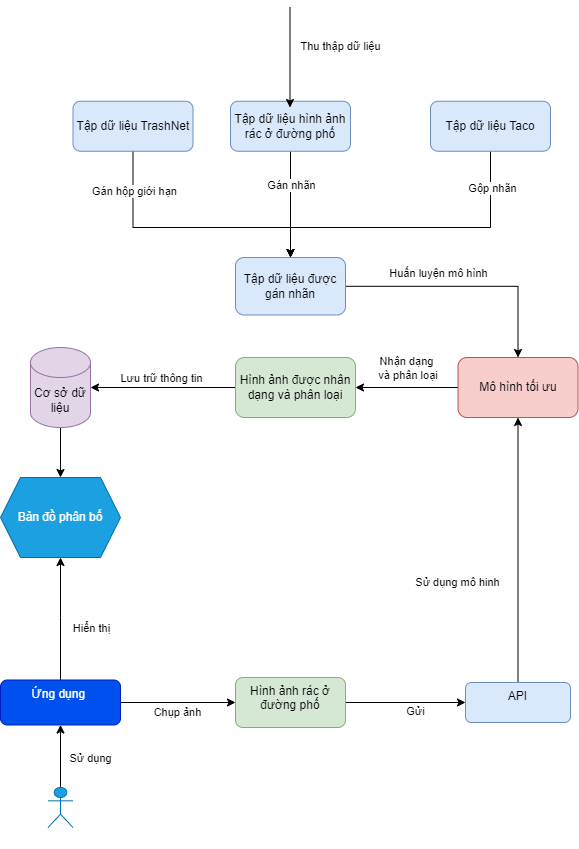
\includegraphics[width=0.8\textwidth]{sodo.png}
	\caption{Sơ đồ hệ thống}
	\label{fig:sodo}
\end{figure}

\end{document}


